\documentclass[tikz,border=4pt]{standalone}
\usetikzlibrary{positioning}

\tikzset{
  unit/.style = {draw, thick, rounded corners=2pt, fill=blue!6,
                 minimum width=26mm, minimum height=9mm, align=center},
  head/.style = {unit, fill=blue!18, font=\bfseries},
}

\begin{document}
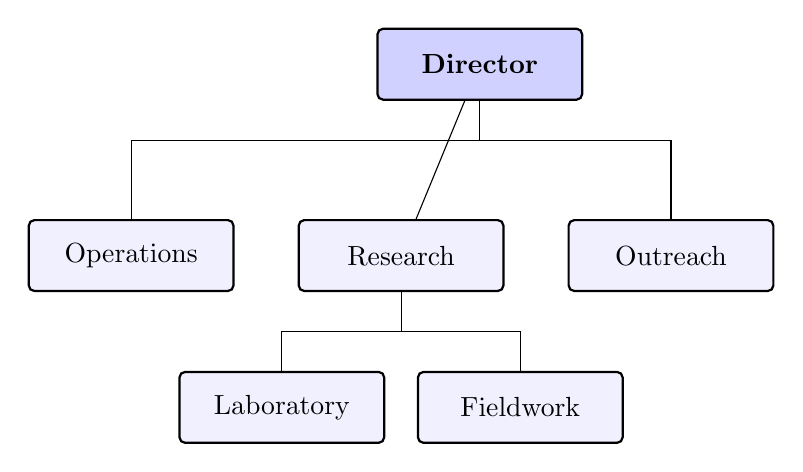
\begin{tikzpicture}[node distance=10mm and 8mm]
  \node[head]                          (director) at (1,0.5)   {Director};
  \node[unit]       (research) at (0,-1.93)   {Research};
  \node[unit, left=of research]        (operations) {Operations};
  \node[unit, right=of research]       (outreach)   {Outreach};
  \node[unit, below left=10mm and 2mm of research.south]  (lab)   {Laboratory};
  \node[unit, below right=10mm and 2mm of research.south] (field) {Fieldwork};

  % Each line drops halfway, then runs across and down: -| turns once.
  \draw (director.south) -- ++(0,-5mm) -| (operations);
  \draw (director)       -- (research);
  \draw (director.south) -- ++(0,-5mm) -| (outreach);
  \draw (research.south) -- ++(0,-5mm) -| (lab);
  \draw (research.south) -- ++(0,-5mm) -| (field);
\end{tikzpicture}
\end{document}
